\section{Auswertung}

\subsection{Fourier-Analyse}

\subsubsection{Rechteck-Spannung}

Die aufgenommenen Messwerte befinden sich in Tabelle \ref{tab:recht}.

\begin{table}[H]
  \centering
  \caption{Messdaten "Rechteck-Spannung"}
  \label{tab:recht}
  \begin{tabular}{S S S}
    \toprule
      {$\nu \:/\: \mathrm{kHz}$} & {$U \:/\: \mathrm{V}$} & {$\frac{U_n}{U_1}$} \\
    \midrule
    400  &	40,8  &  1,000    \\
    800  &	24,6  &  0,603  \\
    1200  &  16,0  &  0,392  \\
    1600  &  11,6  &  0,284  \\
    2000  &  10,8  &  0,265  \\
    2400  &  9,2  &  0,225  \\
    2800  &  7,6  &  0,186  \\
    3200  &  6,0  &  0,147  \\
    3600  &  6,0  &  0,147  \\
    4000  &  5,6  &  0,137  \\
    4400  &  4,8  &  0,118  \\
    \bottomrule
  \end{tabular}
\end{table}
%
%\newpage
%
Aus diesen Messwerten folgt der Graph:

\begin{figure}[H]
  \centering
  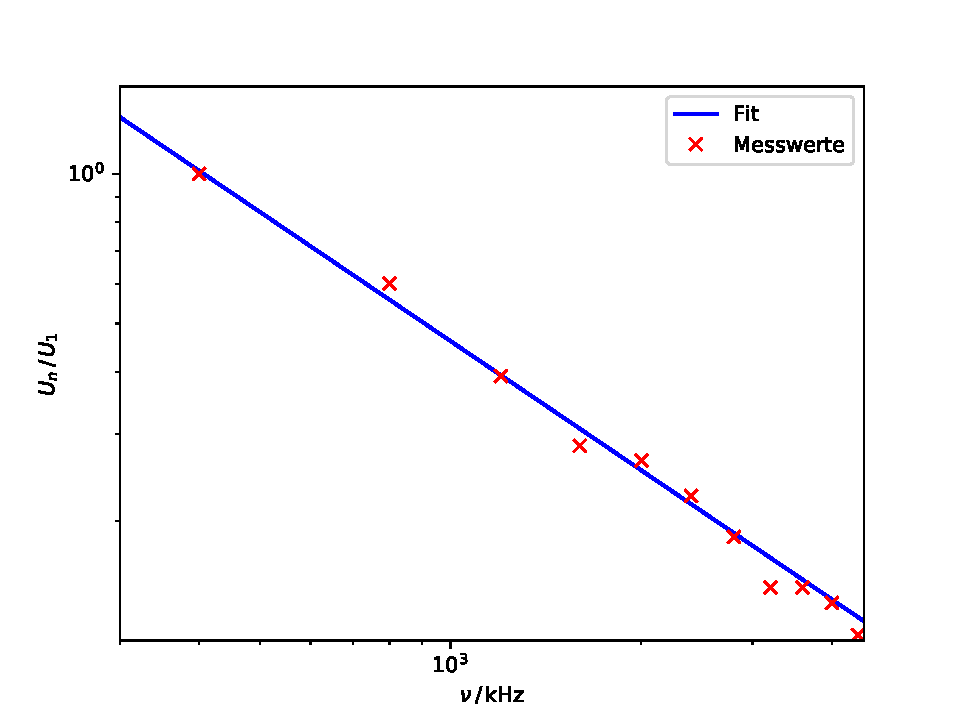
\includegraphics[width=\textwidth]{Plots/recht.pdf}
  \caption{$\frac{U_n}{U_1}$-$\nu$-Diagramm zur Bestimmung der Steigung}
  \label{fig:recht}
\end{figure}

Mithilfe der Messwerte wird die Regression $a \cdot x^{-b}$ durchgeführt, die die Steigung
\begin{equation*}
  b = 0,862 \pm 0,021
\end{equation*}

liefert. Da die Rechteck-Spannung mit $\sfrac{1}{n}$ abfällt, ist der Theoriewert
\begin{equation*}
  b_\text{theo, Rechteck} = 1.
\end{equation*}

Damit ergibt sich eine Abweichung von $\delta_\text{Rechteck} = 13,8 \%$.

% Die Fehler erhält man aus der Gauß'schen Fehlerfortpflanzung
% \begin{equation}
%    \delta = \sqrt{ \sum_{i=1}^{n}(\frac{\partial y}{\partial x_i} \Delta x_i)^2}.
%    \label{eqn:gaus}
%  \end{equation}


\subsubsection{Sägezahn-Spannung}

Die aufgenommenen Messwerte befinden sich in Tabelle \ref{tab:saeg}.

\begin{table}[H]
  \centering
  \caption{Messdaten "Sägezahn-Spannung"}
  \label{tab:saeg}
  \begin{tabular}{S S S}
    \toprule
      {$\nu \:/\: \mathrm{kHz}$} & {$U \:/\: \mathrm{V}$} & {$\frac{U_n}{U_1}$} \\
    \midrule
    87,5  &  226,0  &  1,000    \\
    175,0  &  100,0  & 	0,442  \\
    262,5  &  78,4  &  0,347  \\
    350,0  &  58,4  &  0,258  \\
    437,5  &  42,4  &  0,188  \\
    525,0  &  37,6  &  0,166  \\
    612,5  &  35,2  &  0,156  \\
    700,0  &  28,0  &  0,124  \\
    787,5  &  22,4  &  0,099  \\
    875,0  &  22,4  &  0,099  \\
    962,5  &  21,6  &  0,096  \\
    \bottomrule
  \end{tabular}
\end{table}

Aus diesen Messwerten folgt der Graph:

\begin{figure}[H]
  \centering
  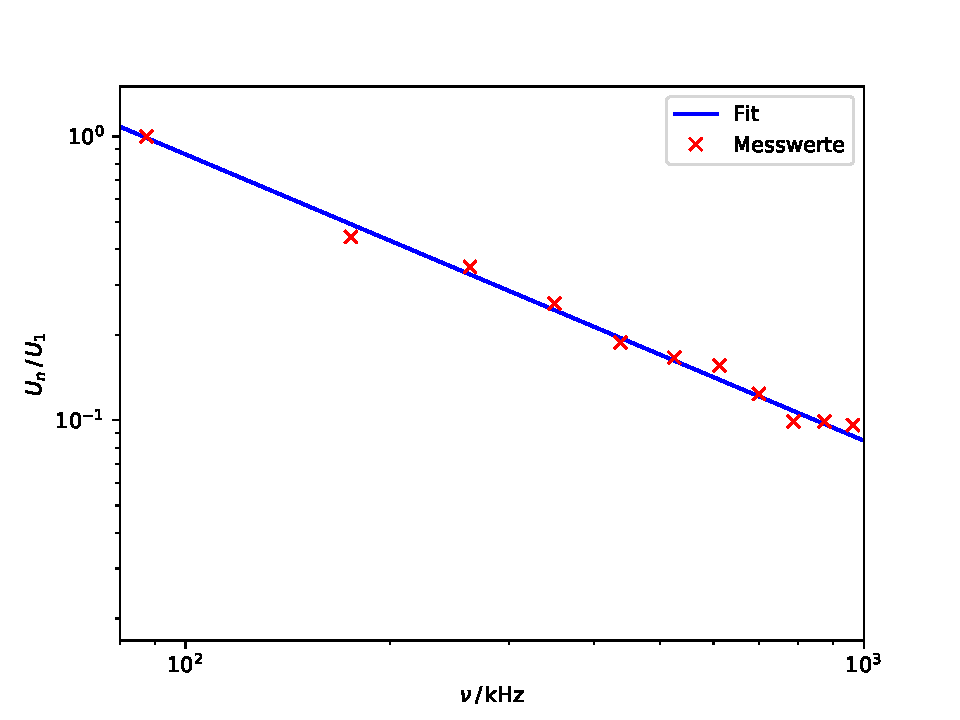
\includegraphics[width=\textwidth]{Plots/saeg.pdf}
  \caption{$\frac{U_n}{U_1}$-$\nu$-Diagramm zur Bestimmung der Steigung}
  \label{fig:saeg}
\end{figure}

Es wird erneut eine Regression durchgeführt. Sie liefert die Steigung
\begin{equation*}
  b = 1,009 \pm 0,027
\end{equation*}

Da auch dieses mal die Spannung mit $\sfrac{1}{n}$ abfällt, ist der Theoriewert wieder
\begin{equation*}
  b_\text{theo, Sägezahn} = 1.
\end{equation*}

Dies ergibt eine Abweichung von $\delta_\text{Sägezahn} = 0,9 \%$.


\subsubsection{Dreieck-Spannung}

Die aufgenommenen Messwerte befinden sich in Tabelle \ref{tab:drei}.

\begin{table}[H]
  \centering
  \caption{Messdaten "Dreieck-Spannung"}
  \label{tab:drei}
  \begin{tabular}{S S S}
    \toprule
      {$\nu \:/\: \mathrm{kHz}$} & {$U \:/\: \mathrm{V}$} & {$\frac{U_n}{U_1}$} \\
    \midrule
    206,2  & 	284,00  &  1,000   \\
    412,4  & 	31,20  & 	0,110  \\
    618,6  & 	12,00  & 	0,042  \\
    824,8  & 	6,16  &  0,022  \\
    1031,0  &  3,12  & 	0,011  \\
    1237,2  &  2,80  & 	0,010  \\
    1443,4  &  1,92  & 	0,007  \\
    \bottomrule
  \end{tabular}
\end{table}

Aus den Messwerten ergibt sich folgende Grafik:

\begin{figure}[H]
  \centering
  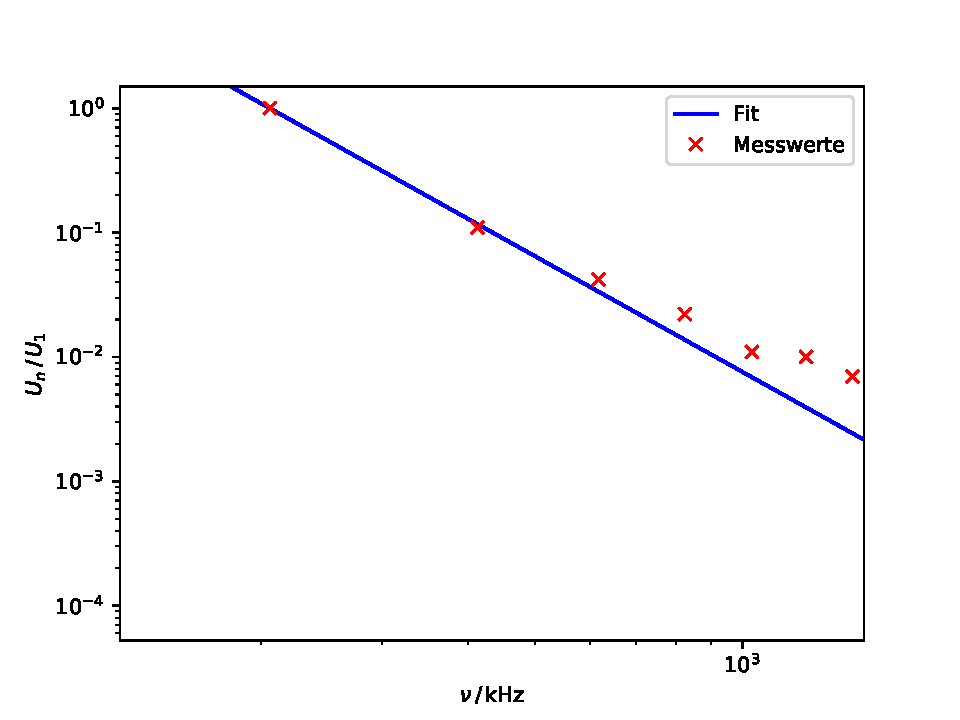
\includegraphics[width=\textwidth]{Plots/drei.pdf}
  \caption{$\frac{U_n}{U_1}$-$\nu$-Diagramm zur Bestimmung der Steigung}
  \label{fig:drei}
\end{figure}

Dieses mal ergibt die Regression die Steigung
\begin{equation*}
  b = 3,093 \pm 0,080
\end{equation*}

Im Gegensatz zu den anderen beiden fällt die Dreieck-Spannung mit $\sfrac{1}{n^2}$ ab.
Der Theoriewert lautet somit
\begin{equation*}
  b_\text{theo, Dreieck} = 2.
\end{equation*}

Die Abweichung beträgt $\delta_\text{Dreieck} = 54,6 \%$.

\subsection{Fourier-Synthese}

\subsubsection{Rechteck-Spannung}

Tabelle \ref{tab:recht2} zeigt die eingestellten Oberwellen, mit denen die Rechteck-Spannung sythetisiert werden soll.

\begin{table}[H]
  \centering
  \caption{Eingestellte Spannungen "Rechteck"}
  \label{tab:recht2}
  \begin{tabular}{c S S S}
    \toprule
    {Oberwelle} & {$U_\text{eingestellt} \,/\, \mathrm{V}$} &
    {$U_\text{theoretisch} \,/\, \mathrm{V}$} & {$\text{Abweichung} \,/\, \%$} \\
    \midrule
    1  &  182,16  &  182,16  & 	0,0  \\
    3  &  59,40  &  60,72  &  2,2  \\
    5  &  35,64  &  36,43  &  2,2  \\
    7  &  27,72  &  26,02  &  6,5  \\
    9  &  19,80  &  20,24  &  2,2  \\
    \bottomrule
  \end{tabular}
\end{table}

Die sich daraus ergebende Rechteck-Spannung, sieht wie folgt aus:

\begin{figure}[H]
  \centering
  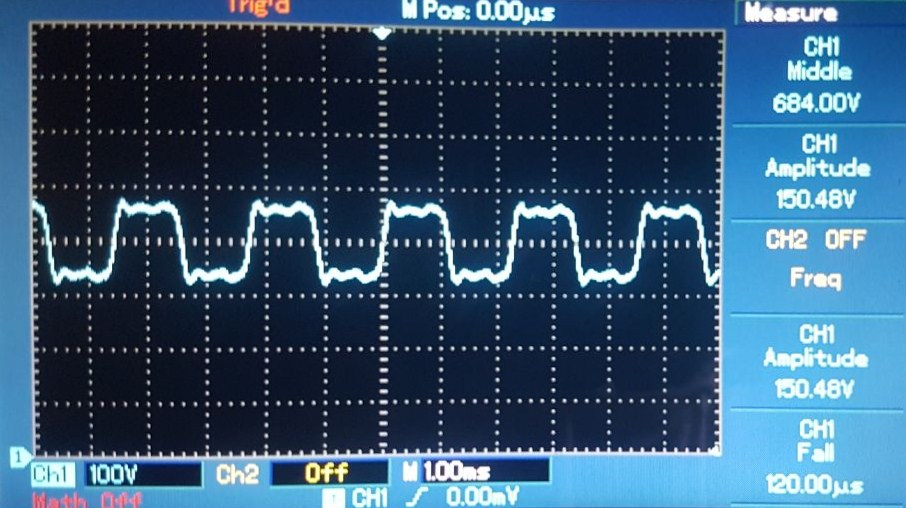
\includegraphics[width=\textwidth]{Text/Bilder/recht.jpg}
  \caption{Synthetisierte Rechteck-Spannung}
  \label{fig:recht2}
\end{figure}

\subsubsection{Sägezahn-Spannung}

Die Sägezahn-Spannung soll aus den in Tabelle \ref{tab:saeg2} aufgeführten Werten synthetisiert werden.

\begin{table}[H]
  \centering
  \caption{Eingestellte Spannungen "Sägezahn"}
  \label{tab:saeg2}
  \begin{tabular}{c S S S}
    \toprule
    {Oberwelle} & {$U_\text{eingestellt} \,/\, \mathrm{V}$} &
    {$U_\text{theoretisch} \,/\, \mathrm{V}$} & {$\text{Abweichung} \,/\, \%$} \\
    \midrule
    1  & 	186,12  &  186,12  & 	0,0 \\
    2  & 	91,08  & 	93,06  & 	2,1  \\
    3  & 	59,40  & 	62,04  & 	4,3  \\
    4  & 	47,52  & 	46,53  & 	2,1  \\
    5  & 	39,60  & 	37,22  & 	6,4  \\
    6  & 	31,68  & 	31,02  & 	2,1  \\
    7  & 	27,72  & 	26,59  & 	4,3  \\
    8  & 	23,76  & 	23,27  & 	2,1  \\
    9  & 	19,80  & 	20,68  & 	4,3  \\
    10  &  15,8  & 	18,61  & 	15,1  \\
    \bottomrule
  \end{tabular}
\end{table}

Es ergibt sich der folgende Spannungsverlauf:

\begin{figure}[H]
  \centering
  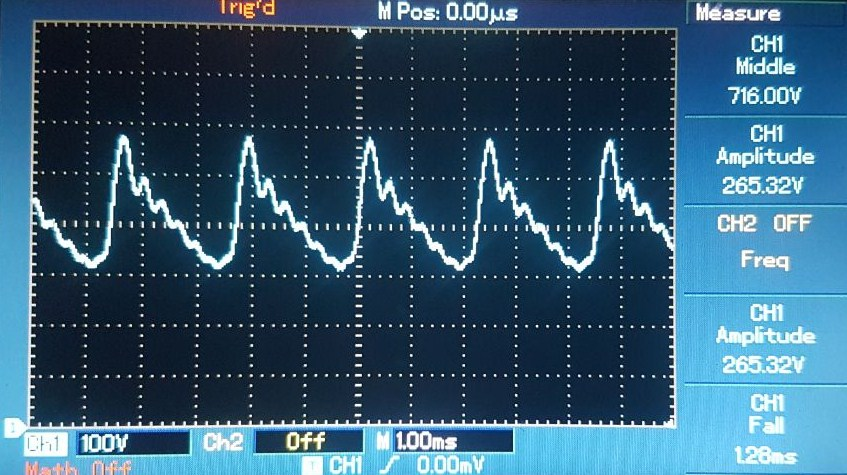
\includegraphics[width=\textwidth]{Text/Bilder/saeg.jpg}
  \caption{Synthetisierte Sägezahn-Spannung}
  \label{fig:saeg2}
\end{figure}

\subsubsection{Dreieck-Spannung}

Die Dreieck-Spannung wird aus den Werten in Tabelle \ref{tab:drei2} synthetisiert.
Da die Dreieck-Spannung mit $\sfrac{1}{n^2}$ abfällt und dadurch die Amplituden sehr schnell sehr klein werden,
war es nicht mehr möglich weitere Oberwellen einzustellen.

\begin{table}[H]
  \centering
  \caption{Eingestellte Spannungen "Dreieck"}
  \label{tab:drei2}
  \begin{tabular}{c S S S}
    \toprule
    {Oberwelle} & {$U_\text{eingestellt} \,/\, \mathrm{V}$} &
    {$U_\text{theoretisch} \,/\, \mathrm{V}$} & {$\text{Abweichung} \,/\, \%$} \\
    \midrule
    1  & 	186,12  &  186,12  & 	0,0 \\
    3  & 	23,76  & 	20,68  & 	14,9 \\
    \bottomrule
  \end{tabular}
\end{table}

Daraus folgt:

\begin{figure}[H]
  \centering
  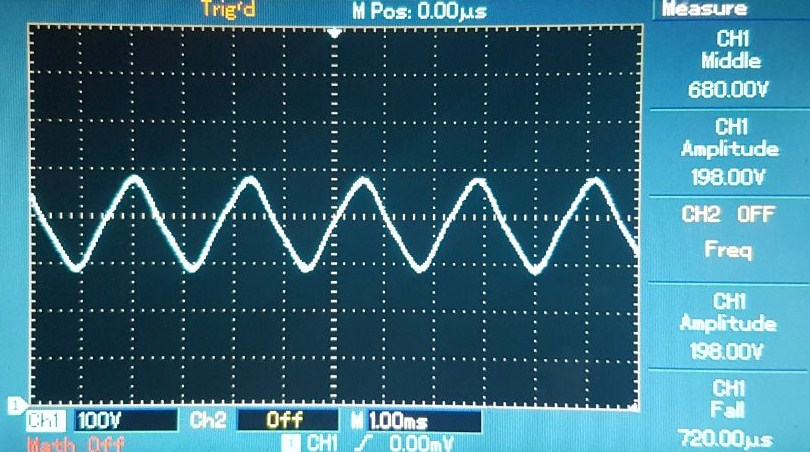
\includegraphics[width=\textwidth]{Text/Bilder/drei.jpg}
  \caption{Synthetisierte Dreieck-Spannung}
  \label{fig:drei2}
\end{figure}
